\section{Exercise 4}
\textit{Our favorite donut shape (torus) has polynomial representation:
$$x^4+2x^2y^2+2x^2z^2−2(r_1^2+r_2^2)x^2+y^4+2y^2z^2+2(r_1^2−r_2^2)y^2+z^4−2(r_1^2+r_2^2)z^2+(r_1^2−r_2^2)^2= 0$$
Could you make a donut shape using poly, or one of the shortcuts? What degree of polynomial should we use}
See \autoref{fig:ex4}.

\begin{figure}[h]
  \centering
  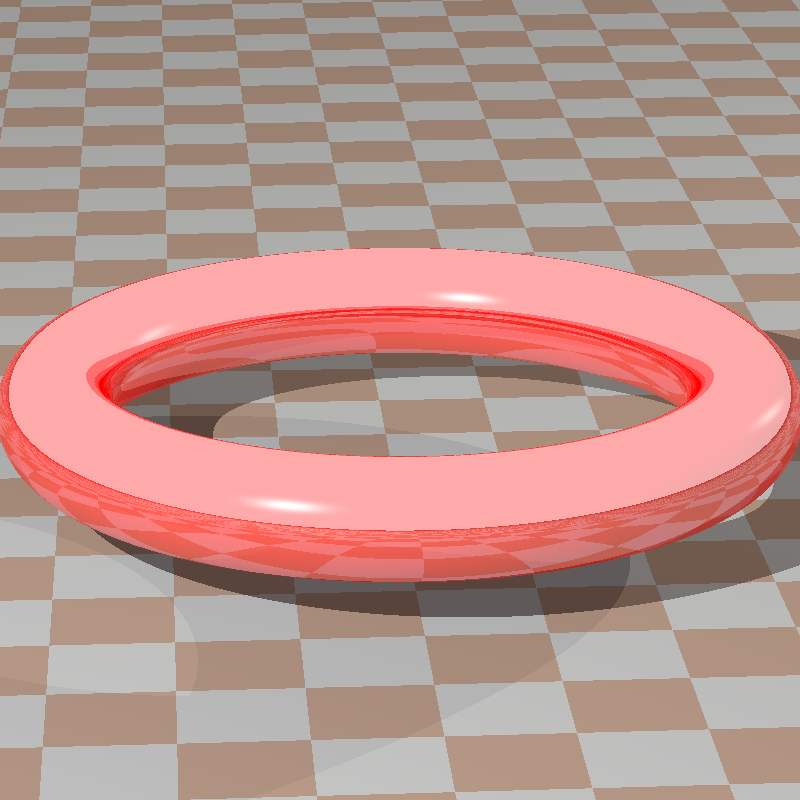
\includegraphics[height=5cm]{ex4.png}
  \caption{Solution for Exercise 4}
  \label{fig:ex4}
\end{figure}